\documentclass[onecolumn,draftclsnofoot, 10pt, compsoc]{IEEEtran}

\usepackage{graphicx}
\usepackage[section]{placeins}
\usepackage{caption}

\usepackage{amssymb}                                         
\usepackage{amsmath}                                         
\usepackage{amsthm}                                

\usepackage{alltt}                                           
\usepackage{float}
\usepackage{color}
\usepackage{url}

\usepackage{balance}
\usepackage[TABBOTCAP, tight]{subfigure}
\usepackage{enumitem}
\usepackage{pstricks, pst-node}
\usepackage{url}
\usepackage{setspace}

\usepackage{etoolbox}
\AtBeginEnvironment{quote}{\singlespacing\vspace{-\topsep}\small}

%\input{pygments.tex}

\usepackage{geometry}
\geometry{left=0.75in,right=0.75in,top=0.75in,bottom=0.75in}
\parindent = 0.0 in
\parskip = 0.1 in


\def \ParSpace{\vspace{.75em}}
\def \Jeremy{			Jeremy Fischer}
\def \Class{		Parallel Programming}
\def \Assn{		Project 5: Vectorized Computation Experiment}
\def \School{	Oregon State University}
\def \Professor{		Matthew Meyn}

\newcommand{\cred}[1]{{\color{red}#1}}
\newcommand{\cblue}[1]{{\color{blue}#1}}

\newcommand{\NameSigPair}[1]{
		\par
		\makebox[2.75in][r]{#1} \hfil 	\makebox[3.25in]{\makebox[2.25in]{\hrulefill} \hfill			
		\makebox[.75in]{\hrulefill}}
		\par\vspace{-12pt} \textit{
			\tiny\noindent
			\makebox[2.75in]{} \hfil		
			\makebox[3.25in]{
				\makebox[2.25in][r]{Signature} \hfill	\makebox[.75in][r]{Date}
			}
		}
}










%%%%%%%%%%%%%%%%%%%%%%%%%%%%%%%%%%%%%%%
\begin{document}
\begin{titlepage}
    \pagenumbering{gobble}
    \begin{singlespace}
    	
\includegraphics[height=4cm]{coe.eps}
        \hfill  
        \par\vspace{.2in}
        \centering
        \scshape{
            \vspace{.5in}
            \textbf{\Large\Assn}\par
            \textbf{\large\Class}\par
            \large{
            	\today \\Spring Term
        	}
            \vfill
            {\large Prepared for}\par
            \huge \School\par
            \vspace{5pt}
            {\Large{\Professor}\par}
            {\large Prepared by }\par

            \vspace{5pt}
            {\Large
                {\Jeremy}\par
            }
            \vspace{20pt}
        }

    \end{singlespace}
\end{titlepage}
\newpage
\pagenumbering{arabic}

% 7. uncomment this (if applicable). Consider adding a page break.
%\listoffigures
%\listoftables
\clearpage





	\section{What machine you ran this on?}
		I ran this on flip.engr.oregonstate.edu.
	
	
	\section{Results Table}
	In the two tables below, the values are the speedup.
	
	\begin{center}
		\textbf{No Vectorization}
	\end{center}
	{ \tabcolsep=1.5pt\relax \begin{tabular}{|c|c|c|c|c|c|c|c|c|}  \hline
		& \textbf{Size: 1000}	& \textbf{Size: 10000}	&  \textbf{Size: 100000} &	\textbf{Size: 1000000}	& \textbf{Size: 2000000}	& \textbf{Size: 15000000}	& \textbf{Size: 30000000} & \textbf{Size: 60000000}
		\\ \hline
		\textbf{Num Threads: 1}	&	1	&	1	&	1	&	1	&	1	&	1	&	1	&	1
		\\ \hline
		\textbf{Num Threads: 2}	&	1.612549713	&	1.974221943	&	0.868688218	&	1.846242111	&	2.719081115	&	2.168886895	&	2.018747843	&	2.035687045
		\\ \hline
		\textbf{Num Threads: 4}	&	3.440045249	&	2.650907556	&	1.711766254	&	5.354409318	&	3.48170106	&	2.406270963	&	2.72296992	&	3.979767133
		\\ \hline
		\textbf{Num Threads: 6}	&	1.82077637	&	3.025776921	&	0.44256159	&	2.09278127	&	4.020273828	&	5.458253571	&	2.879816394	5.&	434650414
		\\ \hline
		\textbf{Num Threads: 8}	&	5.901034929	&	2.217905704	&	1.262473306	&	1.924641148	&	3.543102448	&	3.833063321&		4.226966483	&	4.636038073
		\\ \hline
		\textbf{Num Threads: 16}	&	1.235676554	&	0.811421926	&	0.393096778	&	1.498835585	&	2.525262549&		3.200489279	&	5.154679522	&	6.638708578
		\\ \hline
\end{tabular}}
	\begin{center}
		\textbf{Vectorization}
	\end{center}
	{ \tabcolsep=1.5pt\relax\begin{tabular}{|c|c|c|c|c|c|c|c|c|}  \hline
			& \textbf{Size: 1000}	& \textbf{Size: 10000}	&  \textbf{Size: 100000} &	\textbf{Size: 1000000}	& \textbf{Size: 2000000}	& \textbf{Size: 15000000}	& \textbf{Size: 30000000} & \textbf{Size: 60000000}	\\ \hline
				\textbf{Num Threads: 1}	& 1	& 1	& 1	& 1	& 1	& 1	& 1	& 1
	\\ \hline
				\textbf{Num Threads: 2}	& 0.8886355	& 0.706026308	& 1.210503472	& 0.823988407	& 1.286409852	& 1.217852408	& 0.907975035	& 1.421978833
	\\ \hline
				\textbf{Num Threads: 4}	& 0.352241055	& 1.266392318	& 1.701301342	& 1.942196532	& 0.352786396	& 0.833951131	& 1.128804207	& 1.750934438
	\\ \hline
				\textbf{Num Threads: 6}	& 1.184397163	& 0.522171946	& 0.748858856	& 1.095435685	& 1.057943705	& 1.678185416	& 1.635602748	& 1.563705257
	\\ \hline
				\textbf{Num Threads: 8}	& 0.483557394	& 0.872260015	& 1.646075152	& 0.398297322	& 1.239034483	& 1.740036303	& 1.431946191	& 1.868380629
	\\ \hline
				\textbf{Num Threads: 16}	& 0.228823098	& 0.421822169	& 0.768601874	& 0.692199644	& 1.361885992	& 0.800174203	& 0.936887299	& 2.370013332	\\ \hline
	\end{tabular}}

	
	\section{Results Graph}
	
		
		
		\subsection{No Vectorized Computation}
			\begin{figure}[H]
				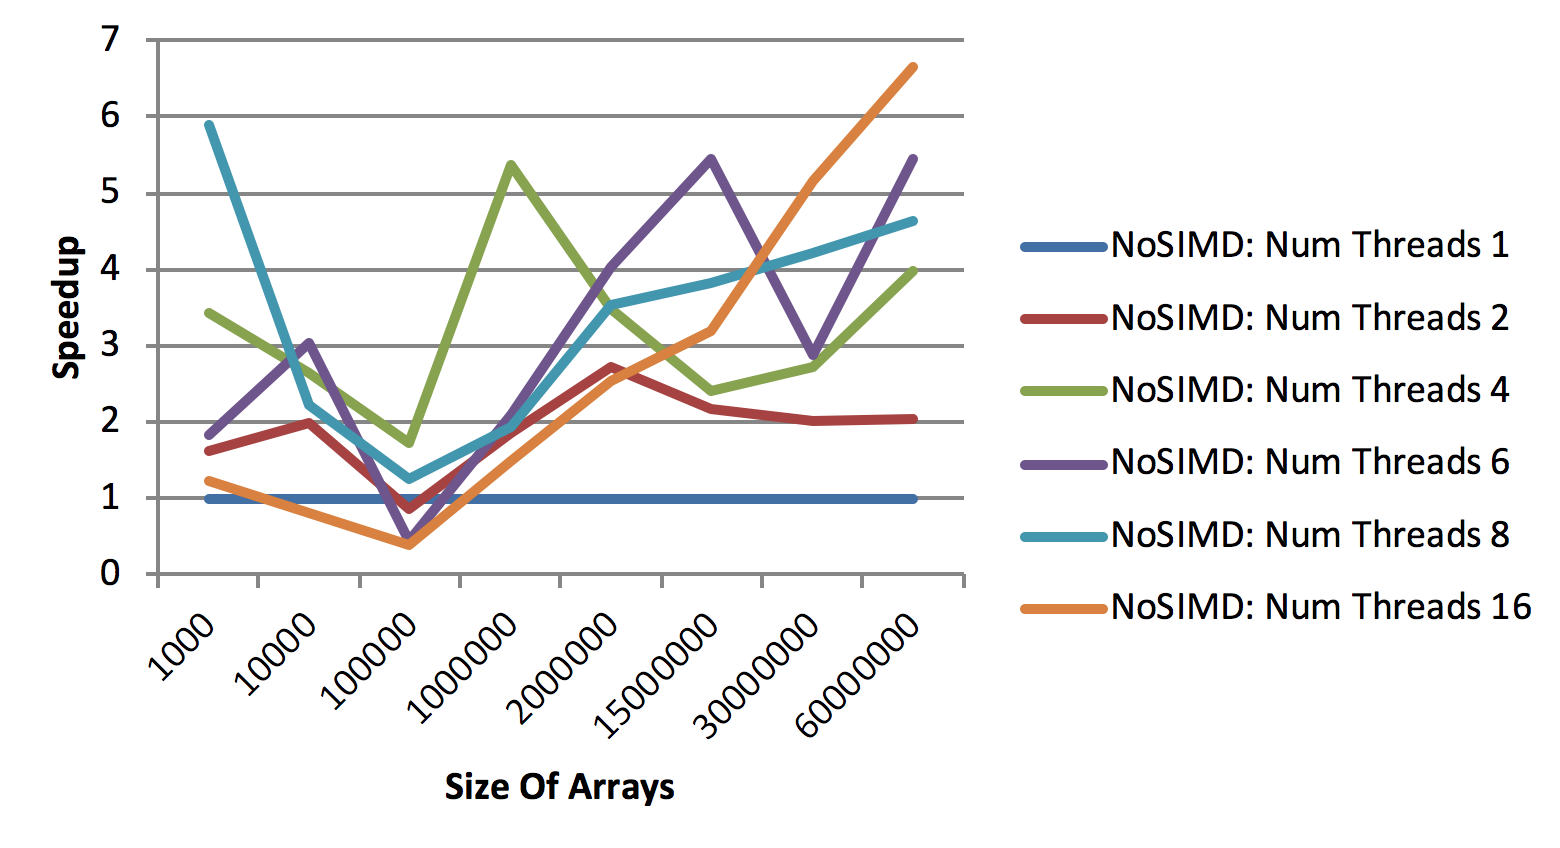
\includegraphics[width=16cm]{noSimSpeedVsNums}
				\centering
				\caption{A graph of the speedup versus the array size. No vectorization}
			\end{figure}
		
		\begin{figure}[H]
			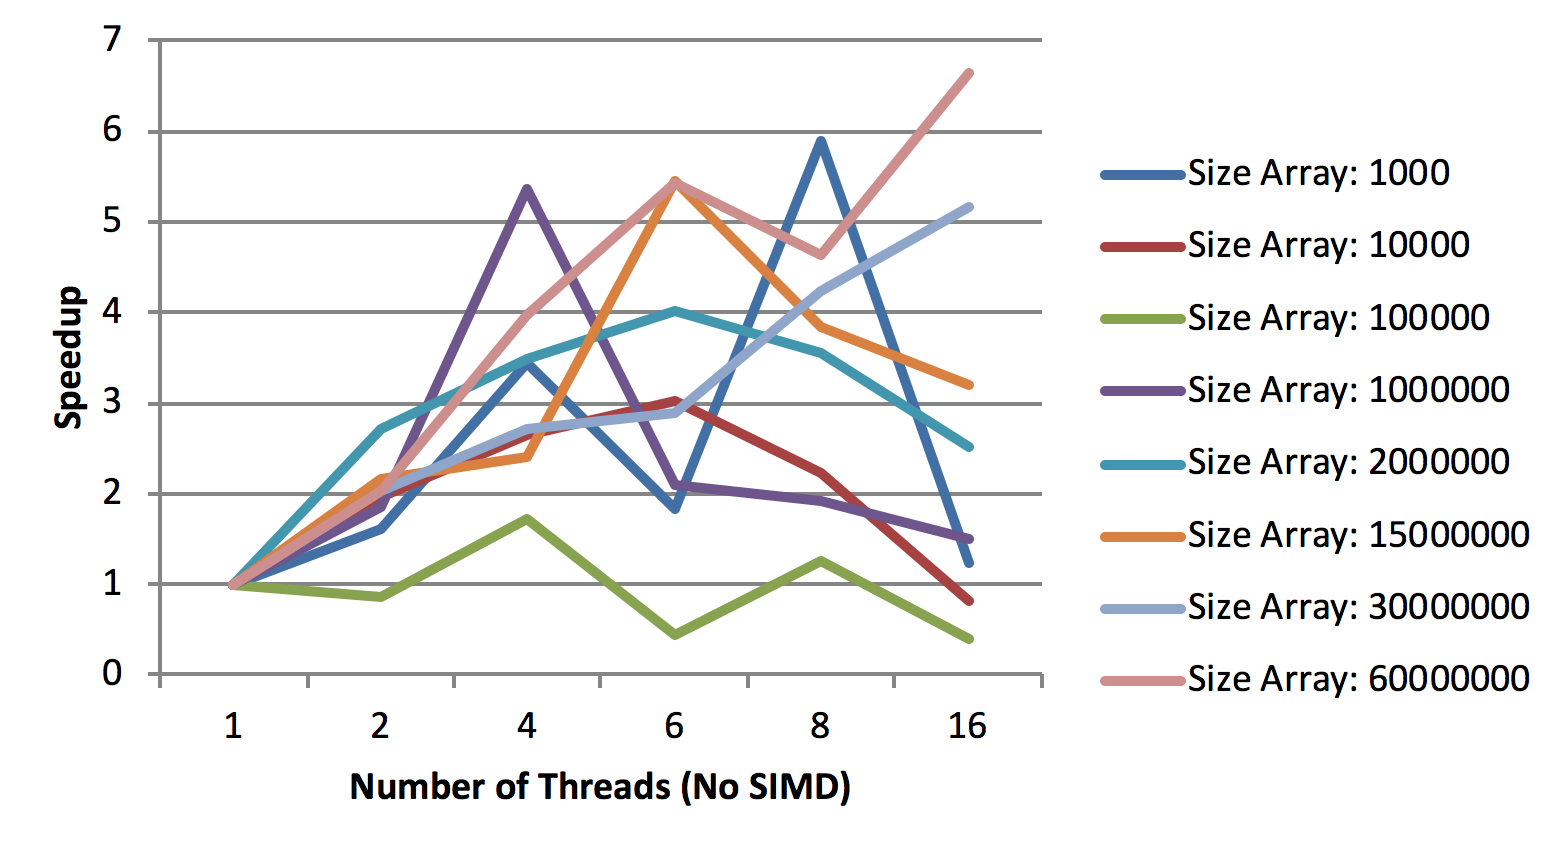
\includegraphics[width=16cm]{noSimSpeedVsThreads}
			\centering
			\caption{A graph of the speedup versus the number of threads. No vectorization}
		\end{figure}
				
				
		\subsection{Vectorized Computation}
			
				\begin{figure}[H]
				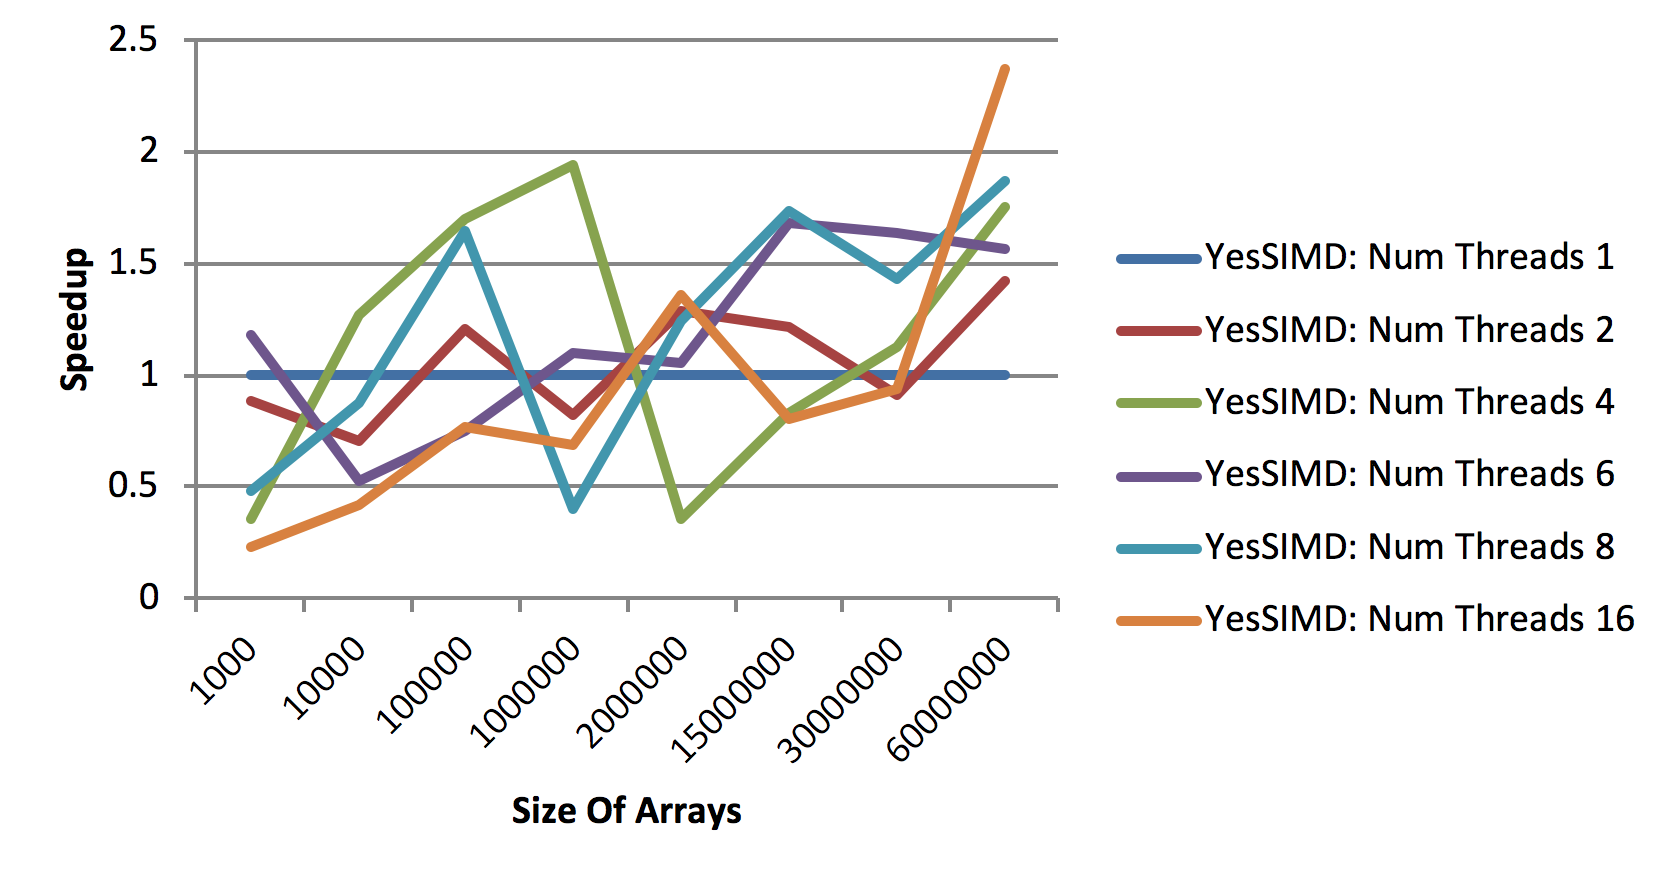
\includegraphics[width=16cm]{yesSimSpeedVsNums}
				\centering
				\caption{A graph of the speedup versus the array size. With vectorization}
			\end{figure}
			
			\begin{figure}[H]
				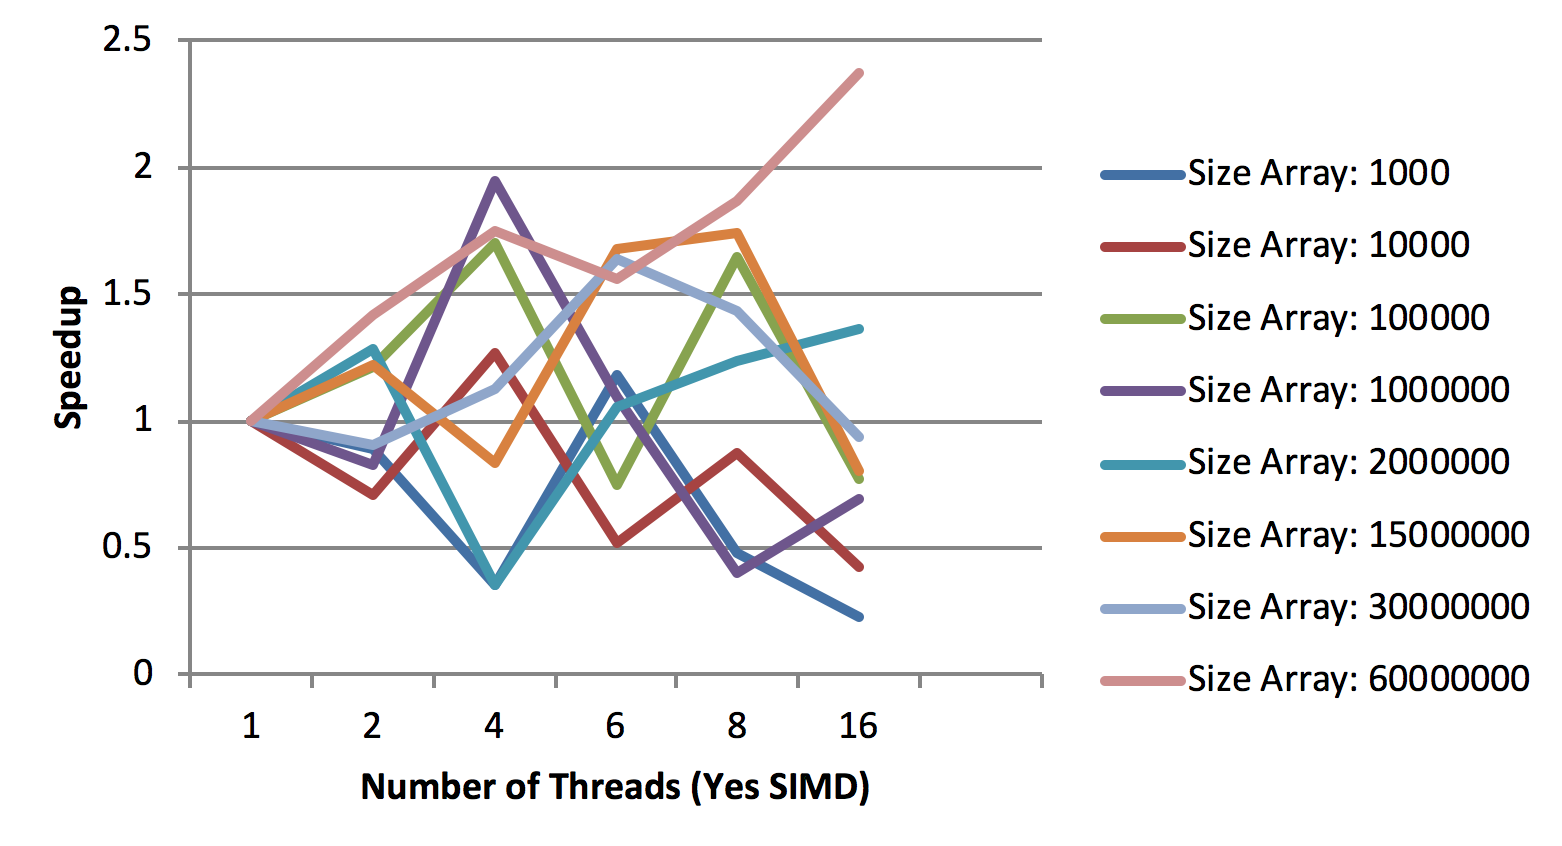
\includegraphics[width=16cm]{yesSimSpeedVsThreads}
				\centering
				\caption{A graph of the speedup versus the number of threads. With vectorization}
			\end{figure}
		
	
	
	\clearpage
	
	\section{What patterns are you seeing in the performance curves?}
		The curves for the non-vectorized simulations reach a higher speedup.
		In the \textit{Speedup vs. Number of Threads (No SIMD)} graph the curves continue to reach higher speedups as the number of threads increases, where in the \textit{Speedup vs. Number of Threads (Yes SIMD)} the speedup tends to decrease as the number of threads increases. Most importantly, in the \textit{Speedup vs. Number of Threads (Yes SIMD)} when there are 16 threads and the size of the arrays is 60 million, the speedup reaches the peak. In all of the graphs, the highest speedup is reached when the size of the arrays is the largest.
	
	
	
	
	\section{Why do you think the patterns look this way?}
		I think that the graphs without vectorization reach higher speedups because all of the increase in speed comes from having more threads. Therefore, the speed gap between one thread versus 16 threads is expected to be large. In the graphs with vectorization the increase in speed comes not only from an increase in the number of threads, but also from the vectorization. One can assume that since the speedups are much larger in the vectorized graphs than the non-vectorized graphs that the performance from adding vectorization is great!
		
		Based off of the sharp peaks in speedup showing up at various points in the \textit{Number of Threads} graphs, this shows that the most efficient choice for the number of threads varies by the array size.
	
	
	
	\section{What does that mean for the proper use of vectorized parallel computing?}
		For the proper use of vectorized parallel computing, the size of the computations should be large. 
		Vectorization also assumes that the computation has no branching or conditional logic.
		The number of threads used along with vectorization is sensitive, so it is important to do some testing to make sure the performance isn't hurting due to the overhead of adding more threads than necessary.



\end{document}